%%%%%%%%%%%%%%%%%%%%%%%%%%%%%%%%%%%%%%%%%%%%%%%%%%%%
% This will help you in writing your homebook
% Remember that the character % is a comment in latex
%
% chapter 3
\chapter{Fetch Stage}
\label{FetchUnit}

The fetch part of the datapath serves to do the operation of obtaining the current instruction.
from the external Instruction Memory (where the program is stored) to then feed it to the subsequent unit of the datapath which decodes the bits.
In this small section there will be the analyzation of the components of the datapath in this respective unit along also the external Memory from which the Instruction Register acquires the data.


\section{Datapath Related Components}

\subsection{ Program Counter Register }
First of all there is the Program Counter Register whose purpose is to store the current address of the instruction inside the Instruction Memory from
which the instruction is fetched. Additionally, this register is synchronous reset and enable to the clock. At reset time, the PC register stores the 
all zero value, meaning that there will always be the fetching of the instruction at the adress 0x00000000 at start up. 
Another important remark is about the signal of input of the PC depends on the outcome of two combinational multiplexers. One multiplexer decides to
feed through the address of the next instruction or the address coming from the output of the ALU in the execute stage. This decision is made on the basis
of a branchStatus signal determined during the Execution Stage, which takes value 1 when a jump or branch needs to be performed.
As a second criteria, we included the second multiplexer to decide if it is needed to stall the PC register or not. This action depends on whether the hazard unit
external to the datapath detects a hazard in the program. In such case it sends a selection signal for this multiplexer set to 1, for making the Program 
counter register assume the same address value in the subsequent clock cycle, so that a stall in the pipelined is formed halting the program.

Additionally, in order to compute the address of the subsequent instruction of the program, a ripple carry adder is used with a fixed operand of one added
to the next instruction.

\subsection{ Instruction Register }

This is the second important register which will store the value of the fetched instruction from the Instruction Memory. like the program counter register,
it has a synchronous enable and a synchronous reset sensitive to rising edges of the clock. The output of this register is propagated and used for the nex important stage,
the decode stage which is explained in the following chapter. 

\subsection{ Next Program Counter }

This important register is placed for the propagation of the subsequent instruction address for the following pipe stages. This way, if the instruction
that was fetched is a jump or a branch, it will be able to compute the address of the jump later on in the execution stage.

\section{External Instruction Memory}

The instruction memory is the memory where all the instructions of the program are stored and it is the component from where the Instruction Register fetches the 
instruction. Upon the presence of an active high reset signal, it loads in a raw format all the thirtytwo bit instructions composing the program. While the reset is zero,
on the basis of the adress that is felt at its input it outputs the associated instruction for the Instruction Register.

In Figure 3.1 is a conceptual drawing which is made to visualize the structure of this component more clearly. the main criterias to consider are that this
memory will always store the first instruction of the program at the all zero address. The second feature of the memory is that it stores the whole instructions
in a row of the memory, this leads to the reason why the addresses are incrememnted by one instead of four, and also it is the reason why the
ripple carry adder adds one instead of four for computing the subsequent instruction's address. We designers made this decision for the purpose of easily creating the
raw memory files while testing the datapath in the early stages. Also another small advantage of this choice is that the minimum required depth of the memory in thi way is exactly the amount
of instructions of the assembly program

\begin{figure}[h!]
    \centering
    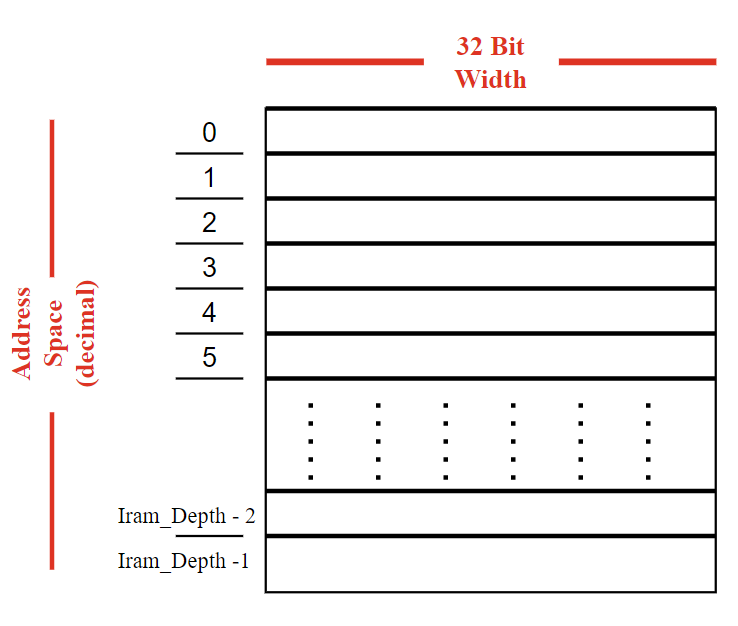
\includegraphics[scale = 0.45]
    {chapters/figures/IRAM}
    \caption{Instruction Memory with addresses separated by one as offset}
    \label{fig:IRAMpic}
    \end{figure}


